\documentclass[11pt]{beamer}
\usepackage[utf8]{inputenc}
\usepackage[T1]{fontenc}
\usepackage{lmodern}
\usepackage{amsmath}
\usepackage{amsfonts}
\usepackage{amssymb}
\usepackage{graphicx}
\usetheme{Boadilla}
\usepackage{media9}
\usepackage{multimedia}
\usepackage{pdfpages}
\usepackage{hyperref}
\usepackage[labelformat=empty]{caption}

\begin{document}
	\author{Julien Nyambal}
	\title{Why GPUs for Deep Learning?}
	%\subtitle{}
	\logo{capitec}
	\institute{Capitec Bank}
	\logo{
\includegraphics[height=0.5cm]{capitec.png}}
	%\date{}
	\setbeamertemplate{navigation symbols}{}
	\begin{frame}[plain]
		\maketitle
	\end{frame}

\begin{frame}
	\centering
	While a CPU is the brains of a computer, GPU is its soul ... Nvidia
\end{frame}

	\begin{frame}
		\frametitle{What will be covered ...}
		\tableofcontents
	\end{frame}

\section{What is Machine Learning?}
\begin{frame}
	\frametitle{What is Machine Learning?}
	\begin{figure}
		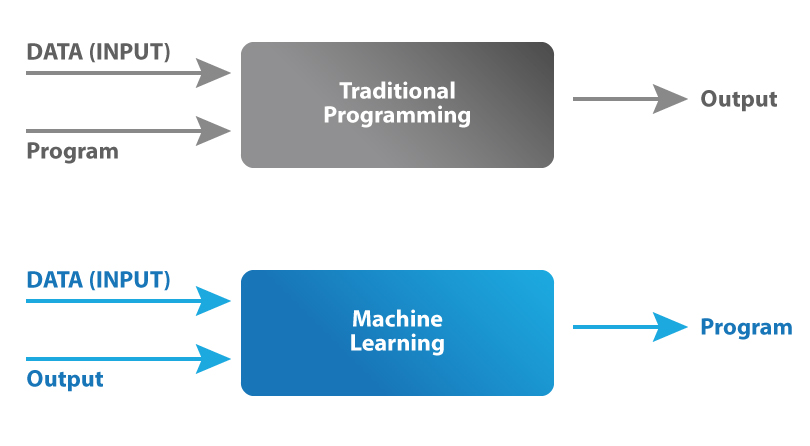
\includegraphics[width=100mm,scale=0.7]{ml}
		\caption{A general definition of a ML}
	\end{figure}
\end{frame}

\begin{frame}
	\frametitle{What is Machine Learning?: Conceptual Overview}
	\begin{figure}
	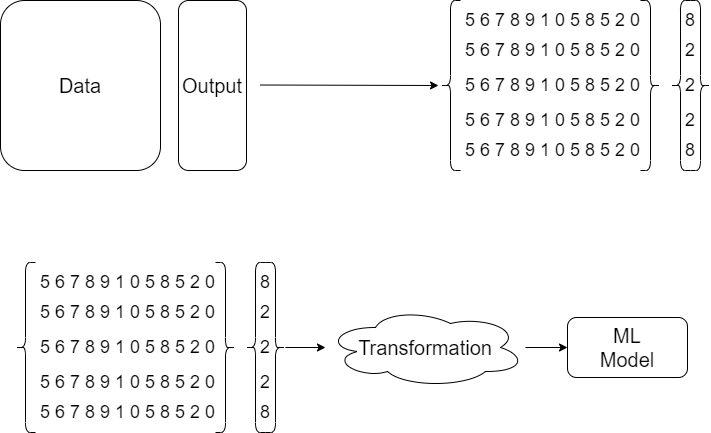
\includegraphics[width=100mm,scale=0.7]{ml_concept}
	\caption{ML - Conceptual}
\end{figure}
\end{frame}

\begin{frame}
	\frametitle{What is Machine Learning?: Deep Learning}
	\begin{figure}
		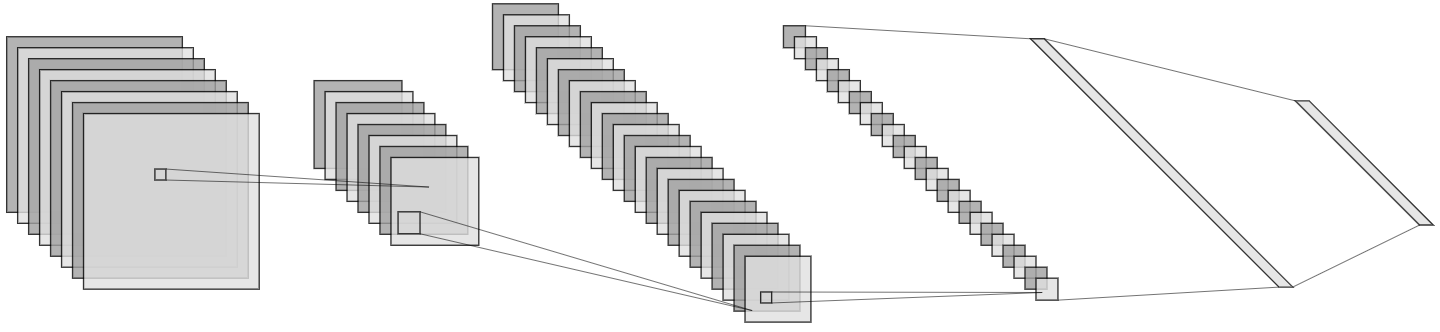
\includegraphics[width=55mm,scale=0.5]{cnn}\hspace{2mm}
		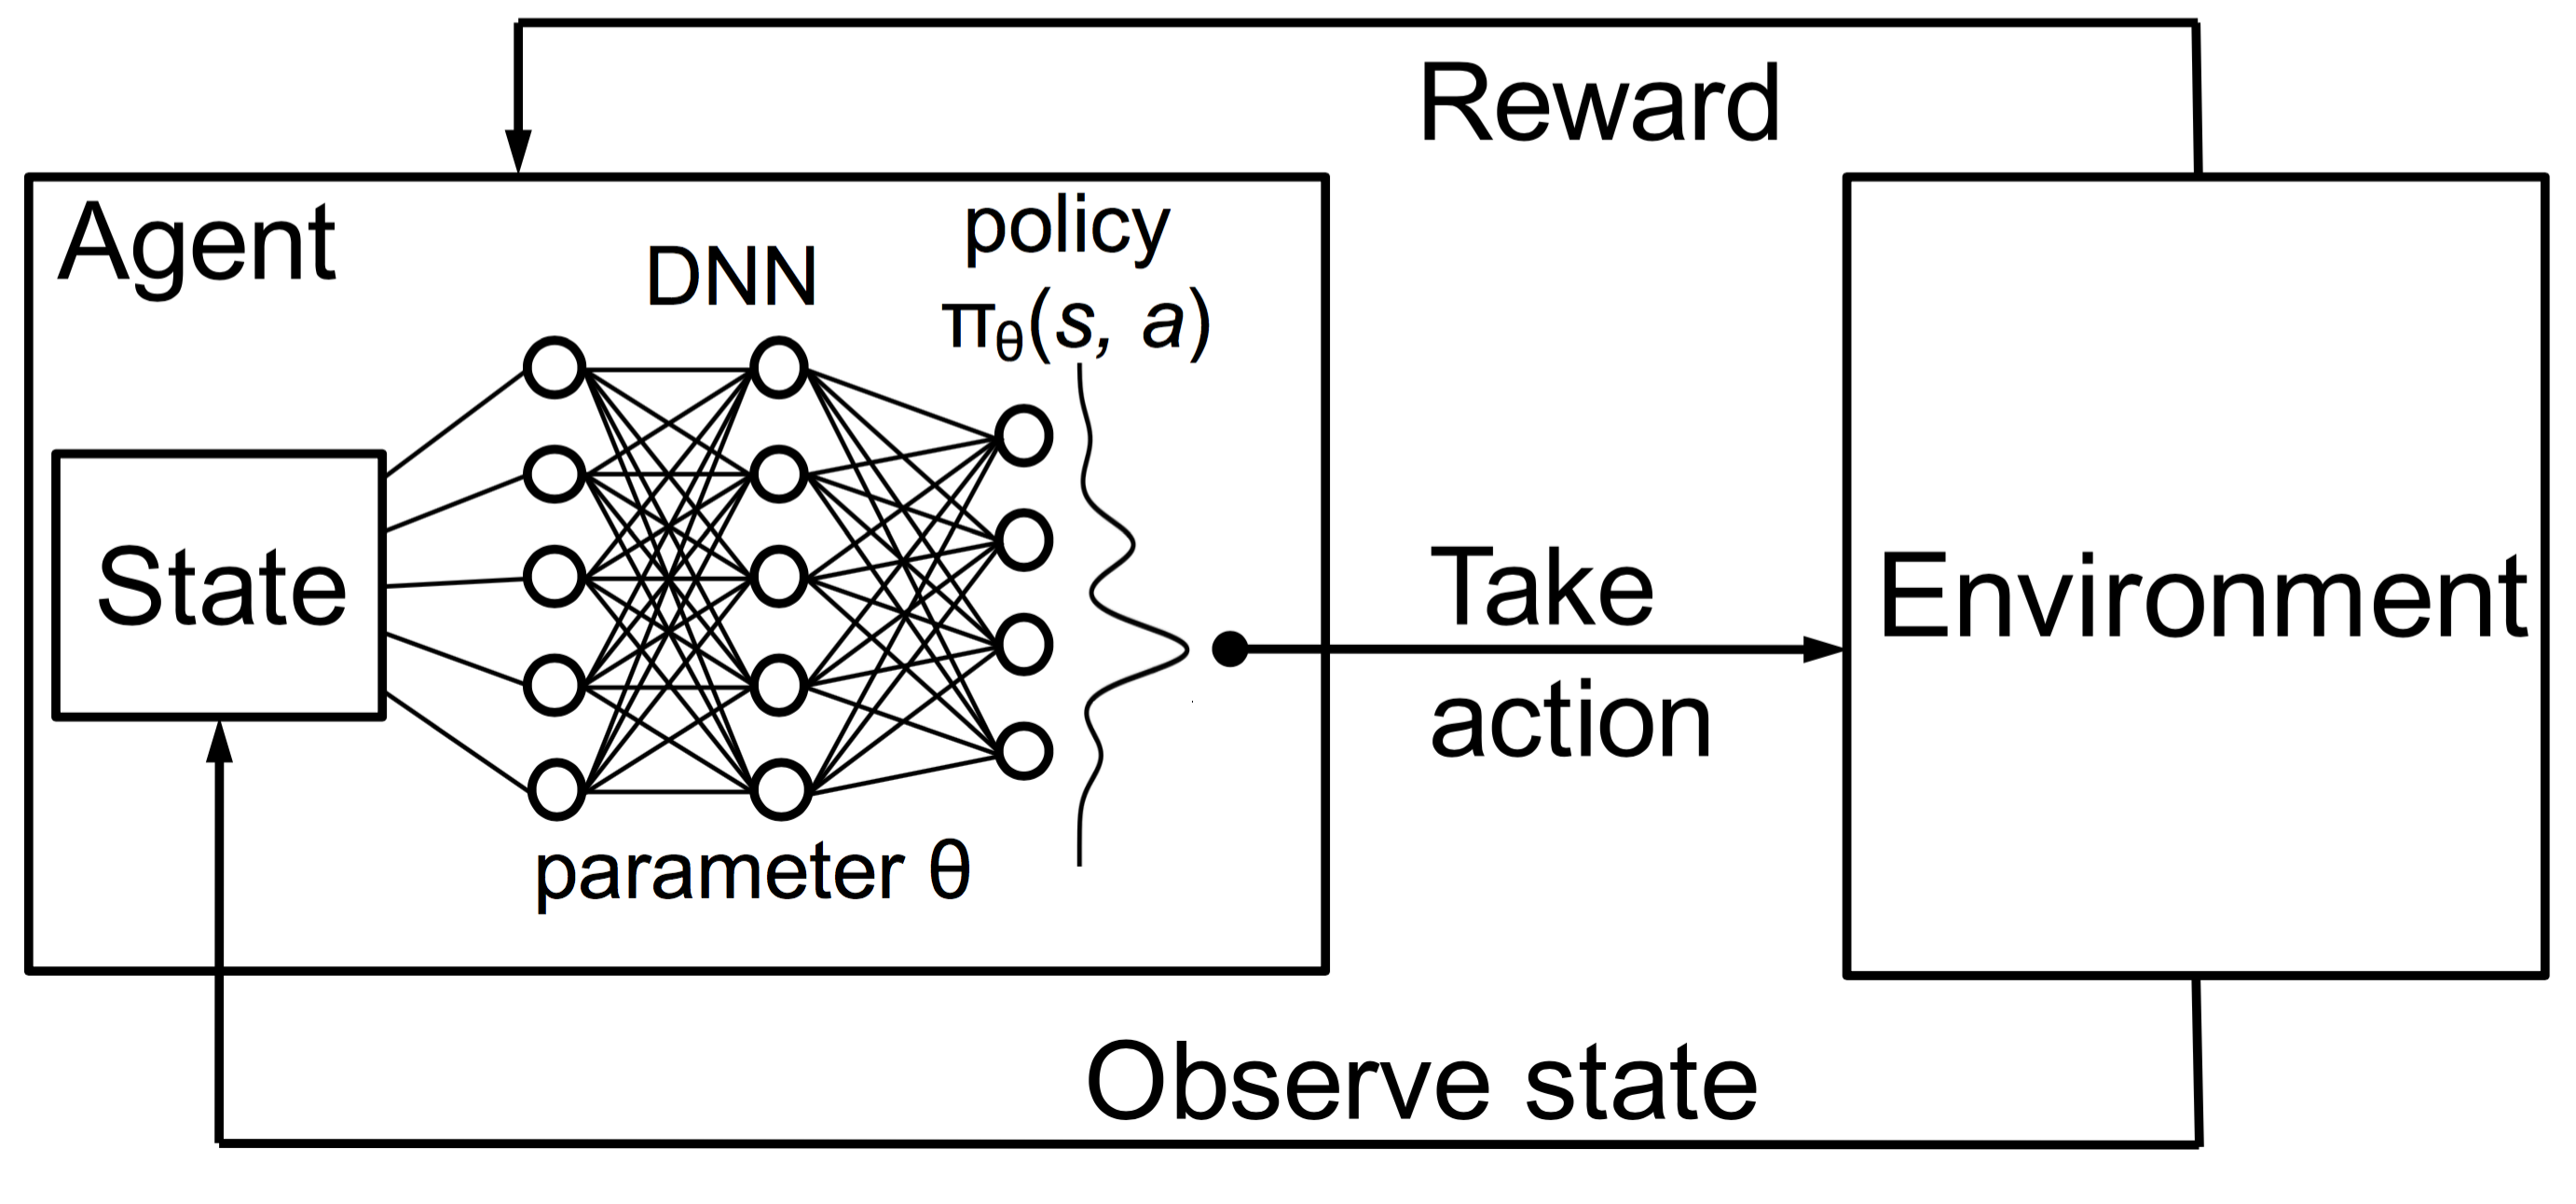
\includegraphics[width=55mm,scale=0.5]{drl}
		\\[\smallskipamount]
		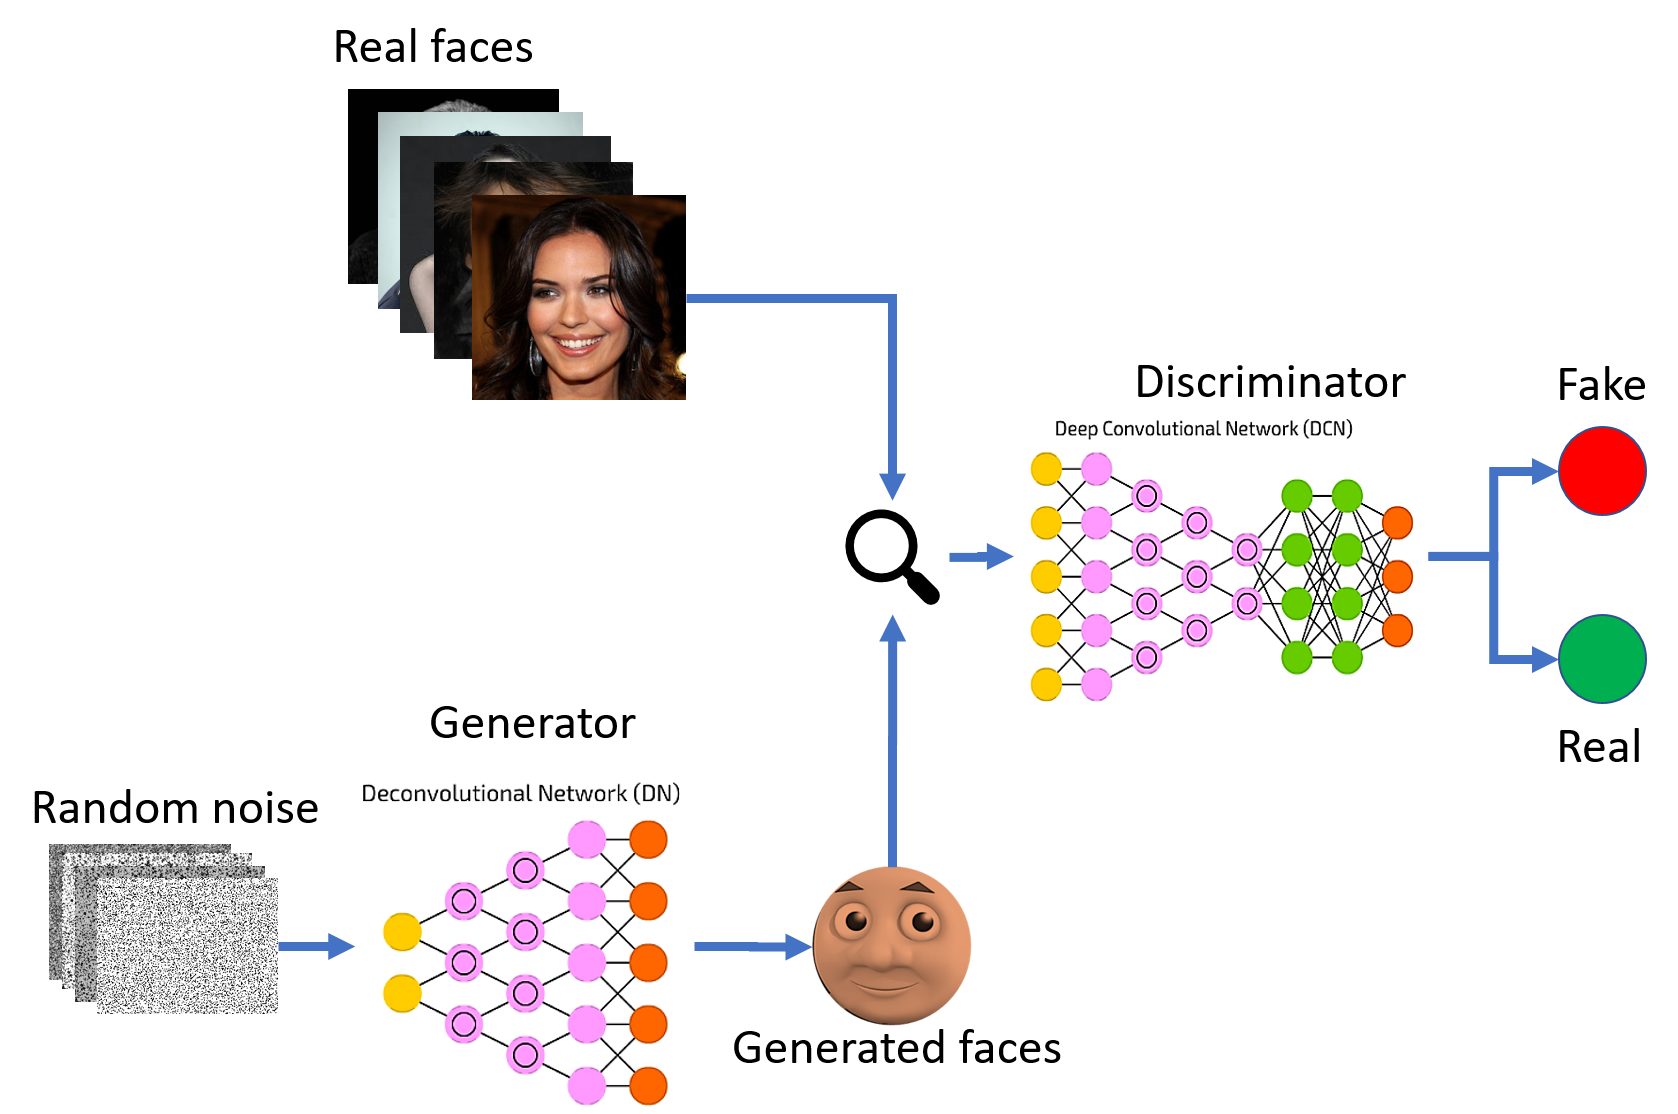
\includegraphics[width=55mm,scale=0.5]{gan}\hspace{2mm}
		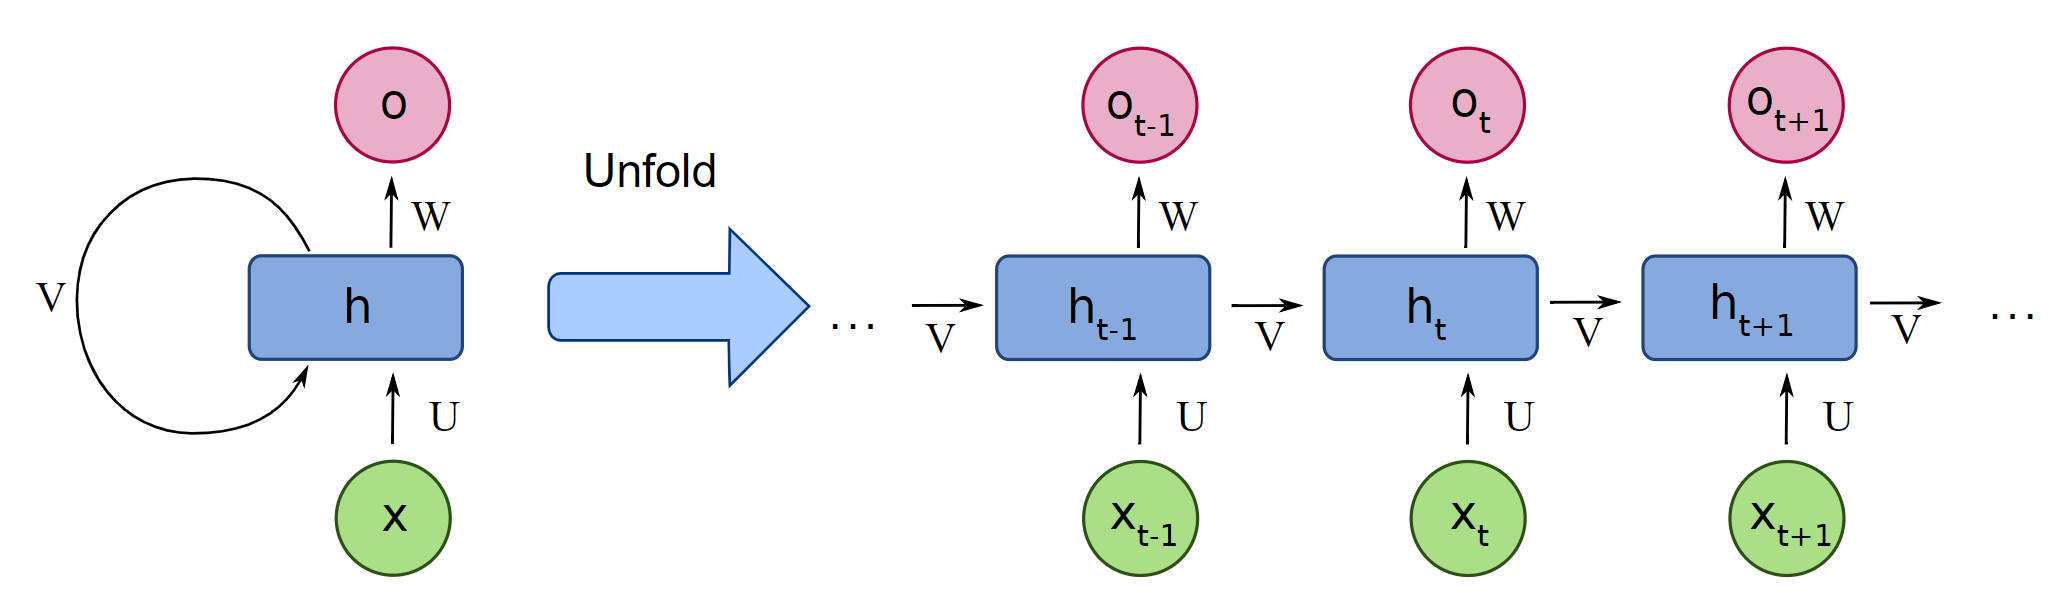
\includegraphics[width=55mm,scale=0.5]{rnn}
	\end{figure}
\end{frame}

\section{RAM, CPU, GPU, TPU}
\subsection{Description}
\begin{frame}
	\frametitle{RAM, GPU, CPU, TPU}
	\begin{center}
		\tiny
	\begin{tabular}{| c | p{2.5cm}| p{2.5cm} | p{2.5cm} | }
		\hline
		\textbf{Acronym} & \textbf{Central Processing Unit}  & \textbf{Graphical Processing Unit}& \textbf{Tensor Processing Unit} \\
		\hline
		\textbf{Description} & Performs basic logic, arithmetic, and I/O operations, and allocate commands to other components and subsystems running in a computer. It is the orchestrator of the other hardware components of the computer system, including the GPU. Most systems have \textbf{a shared GPU resource for basic display}.& \textbf{Dedicated} device designed specifically to accelerate computer graphics workloads, particularly for 3D graphics. While they are still used for their original purpose of accelerating graphics rendering, GPU parallel computing is now used in a wide range of applications, including graphics and video rendering.  & Google’s custom-developed application-specific integrated circuits used to accelerate \textbf{machine learning} workloads, by accelerating the performance of linear algebra computations.   Like a dedicated \href{https://cloud.google.com/tpu/docs/intro-to-tpu}{\textit{\textbf{Machine Learning CPU}}}(link) \\
		\hline
		\textbf{Processing style} & Sequential (But multitask) & Distributed (Given a single heavy-duty load)  & Distributed  \\
		\hline
		\textbf{Graphic Rendering API} & OpenCL& CUDA (Nvidia) & TPU Machine Instructions  \\
		\hline
		\textbf{Specialty} & Orchestrating several tasks performed by the OS &	\begin{itemize}
			\item Graphically intense video game Image Rendering
			\item Distributed Complex matrix operation: \textbf{Machine Learning} and \textbf{HPC}
			\item Video Editing 
		\end{itemize} & Handles very specific mathematical operations: \begin{itemize}
		\item Matrix Multiply Unit (MXU) which runs matrix multiplications 
		\item Vector Processing Unit (VPU) for all other tasks such as activations, softmax, ...
	\end{itemize}\\
		\hline  
	\end{tabular}
\end{center}
\end{frame}

\subsection{TPU: Tensor Processing Unit}
\begin{frame}
	\frametitle{RAM, GPU, CPU, TPU}
	\begin{figure}
		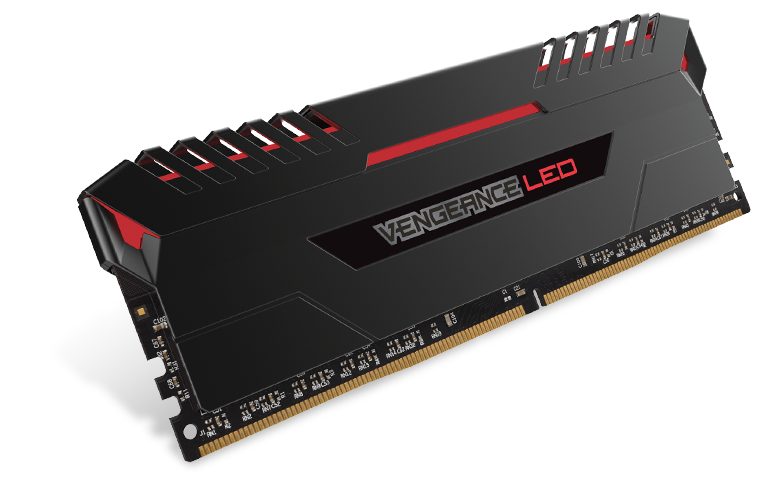
\includegraphics[width=50mm,scale=0.5]{ram5}\hspace{2mm}
		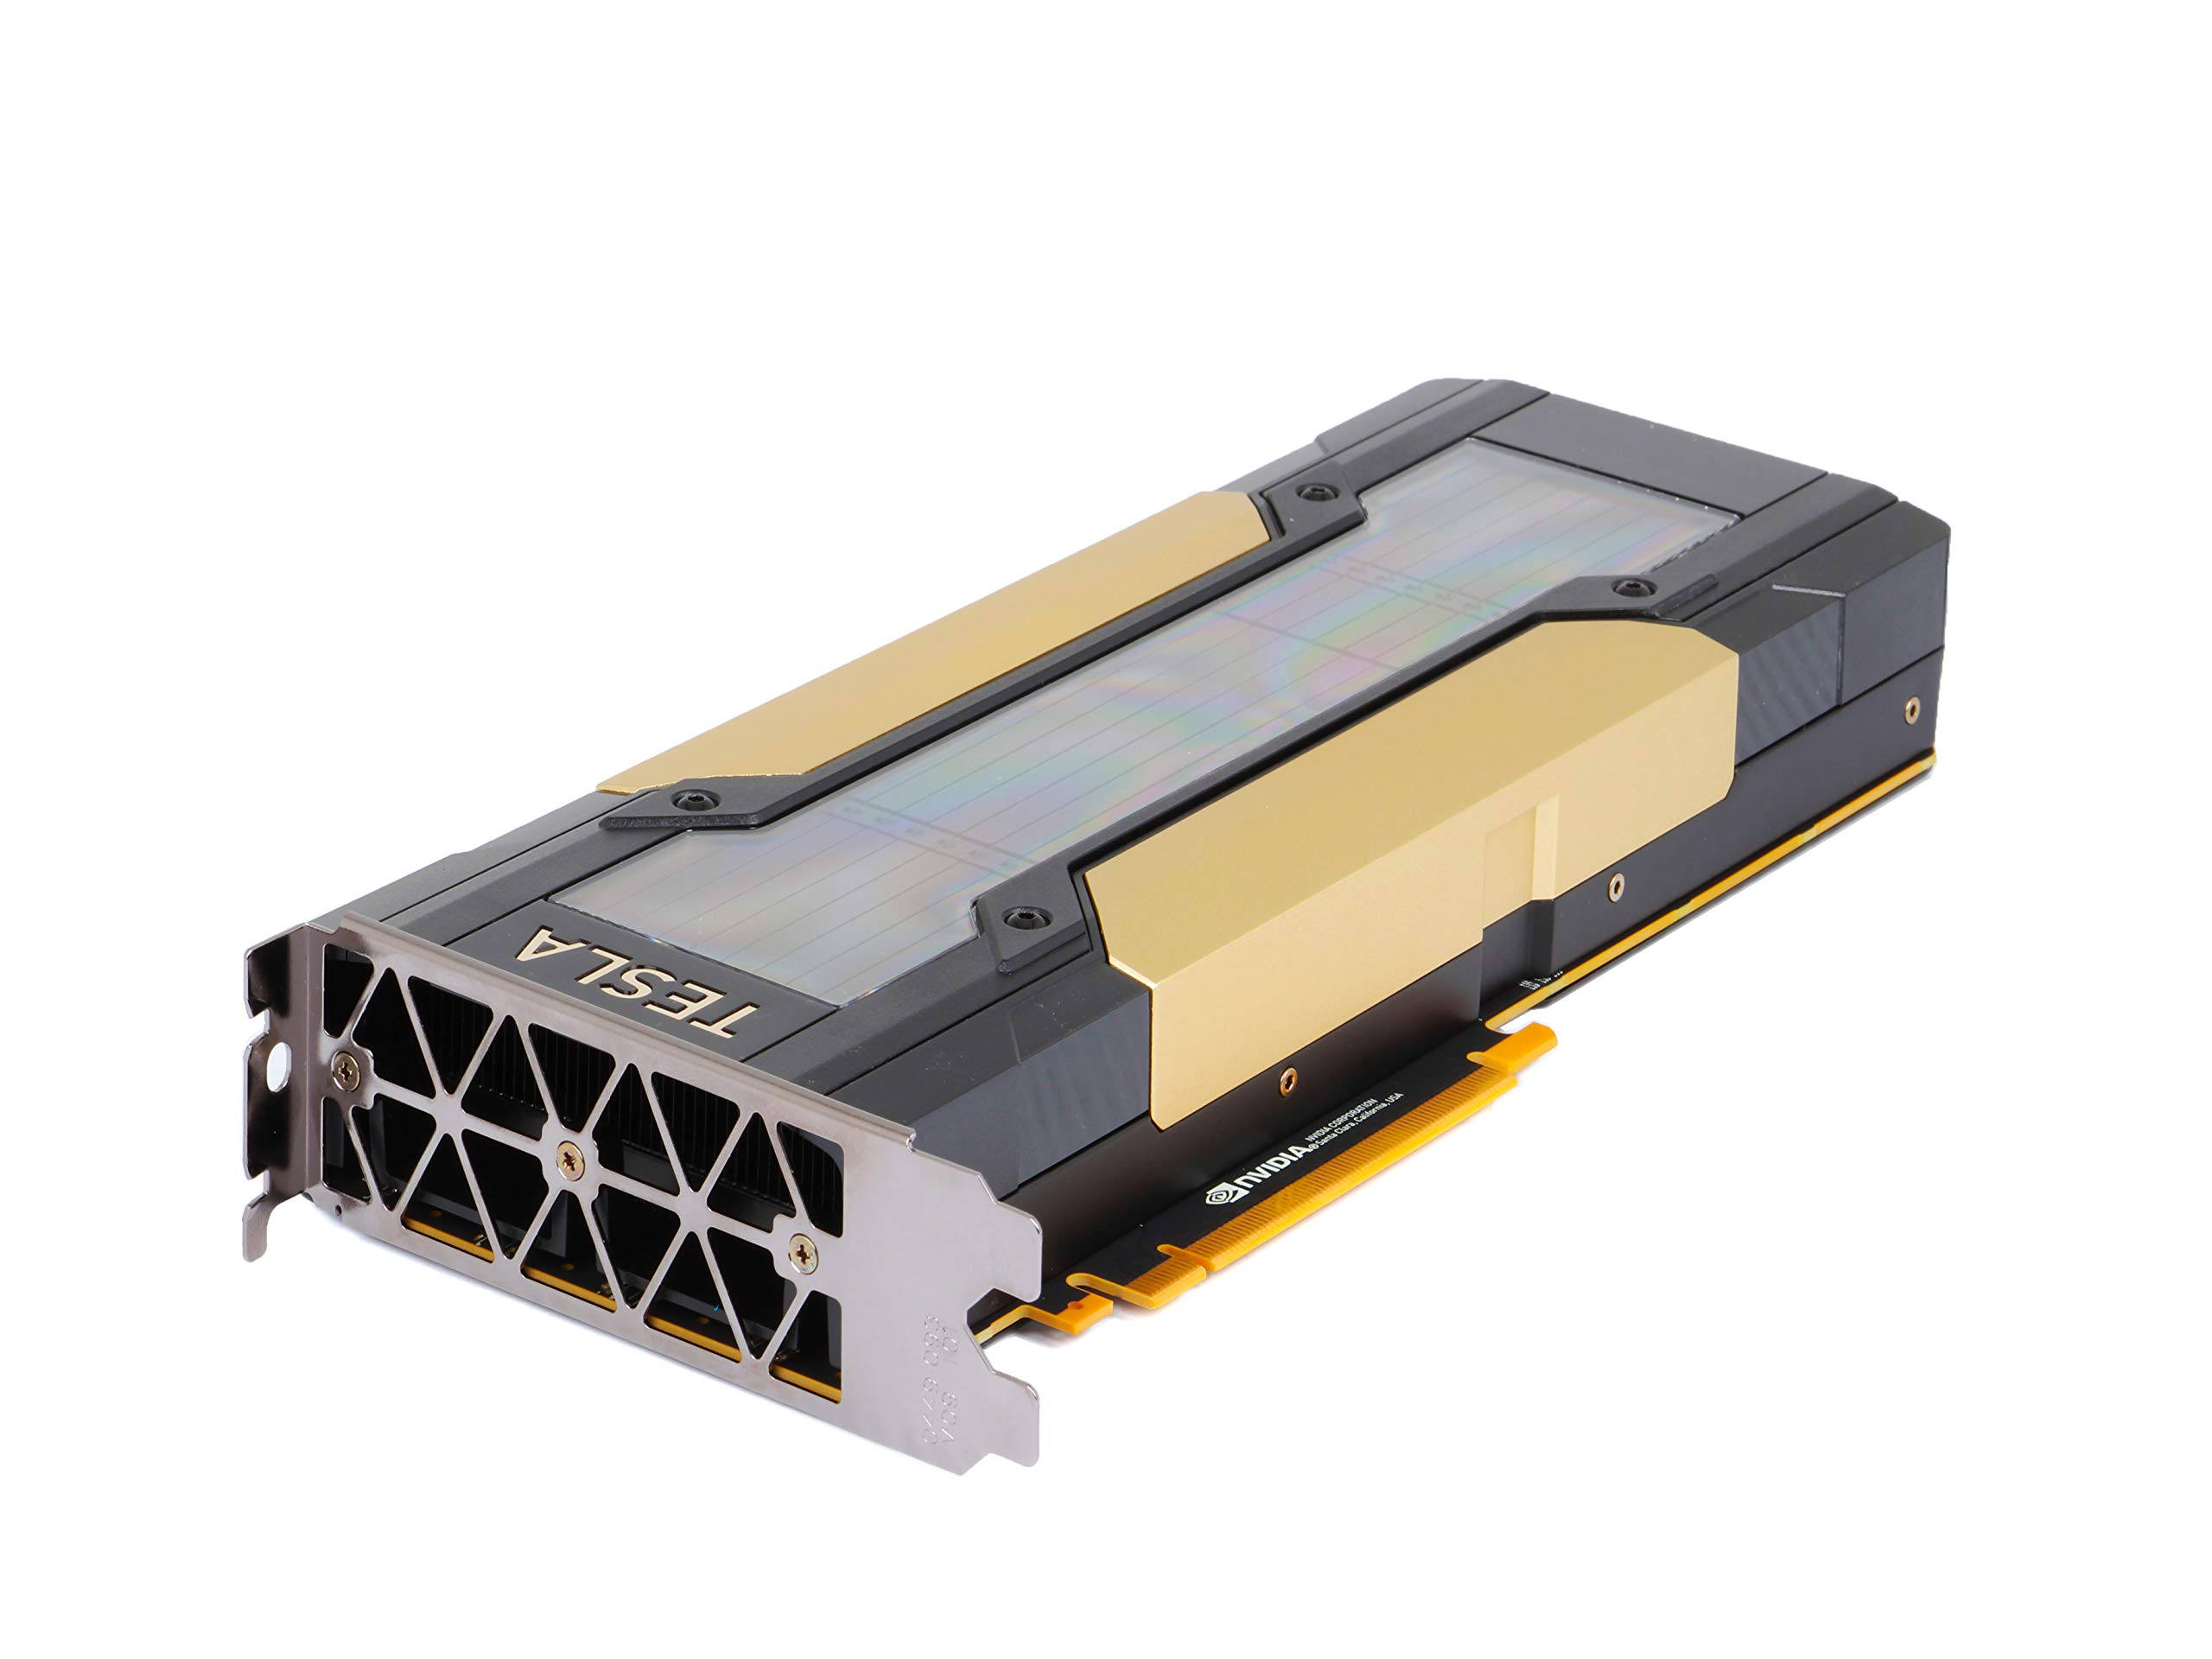
\includegraphics[width=50mm,scale=0.5]{v100}
		\\[\smallskipamount]
		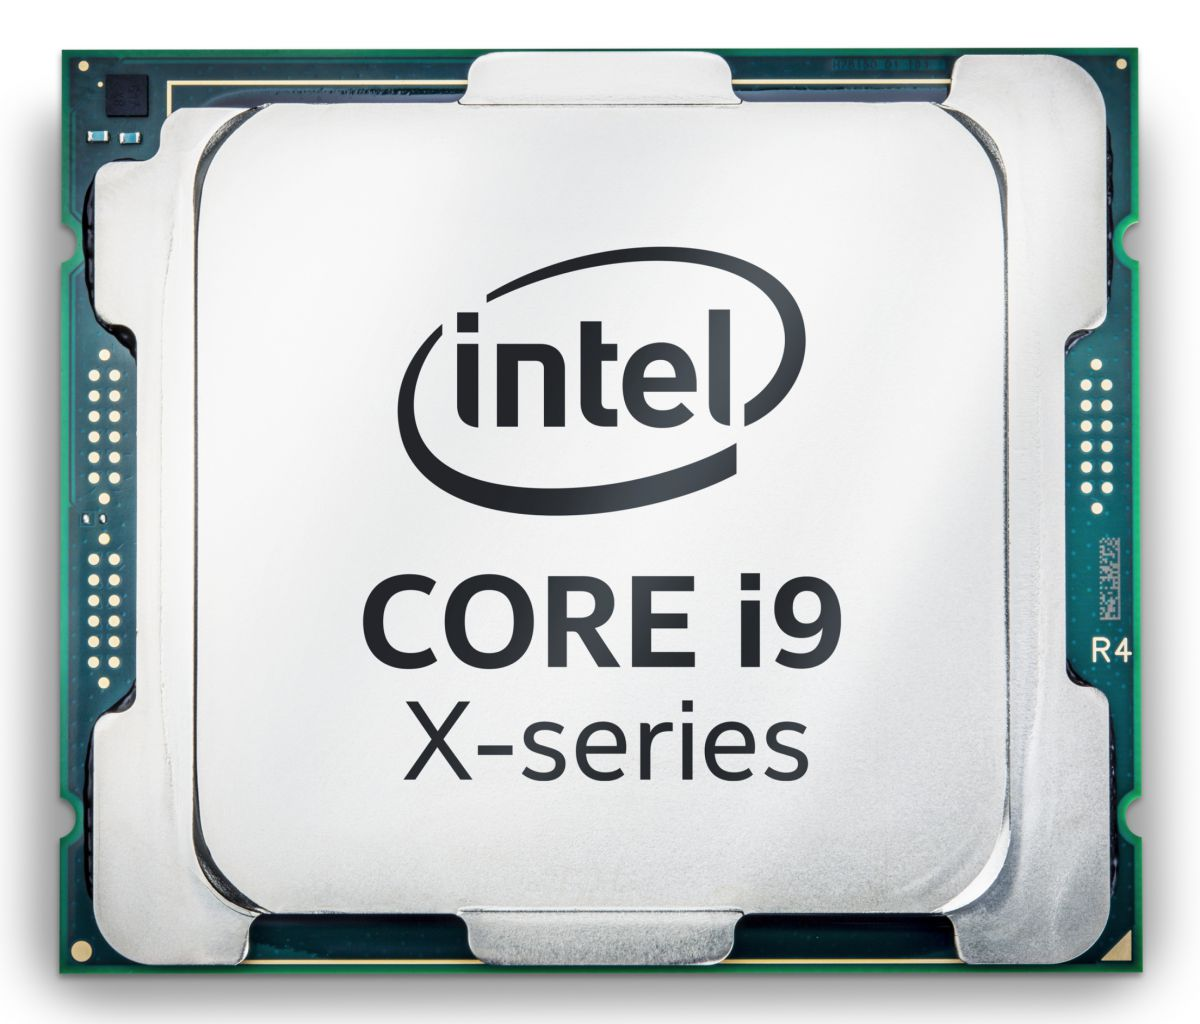
\includegraphics[width=50mm,scale=0.5]{cpu2}\hspace{2mm}
		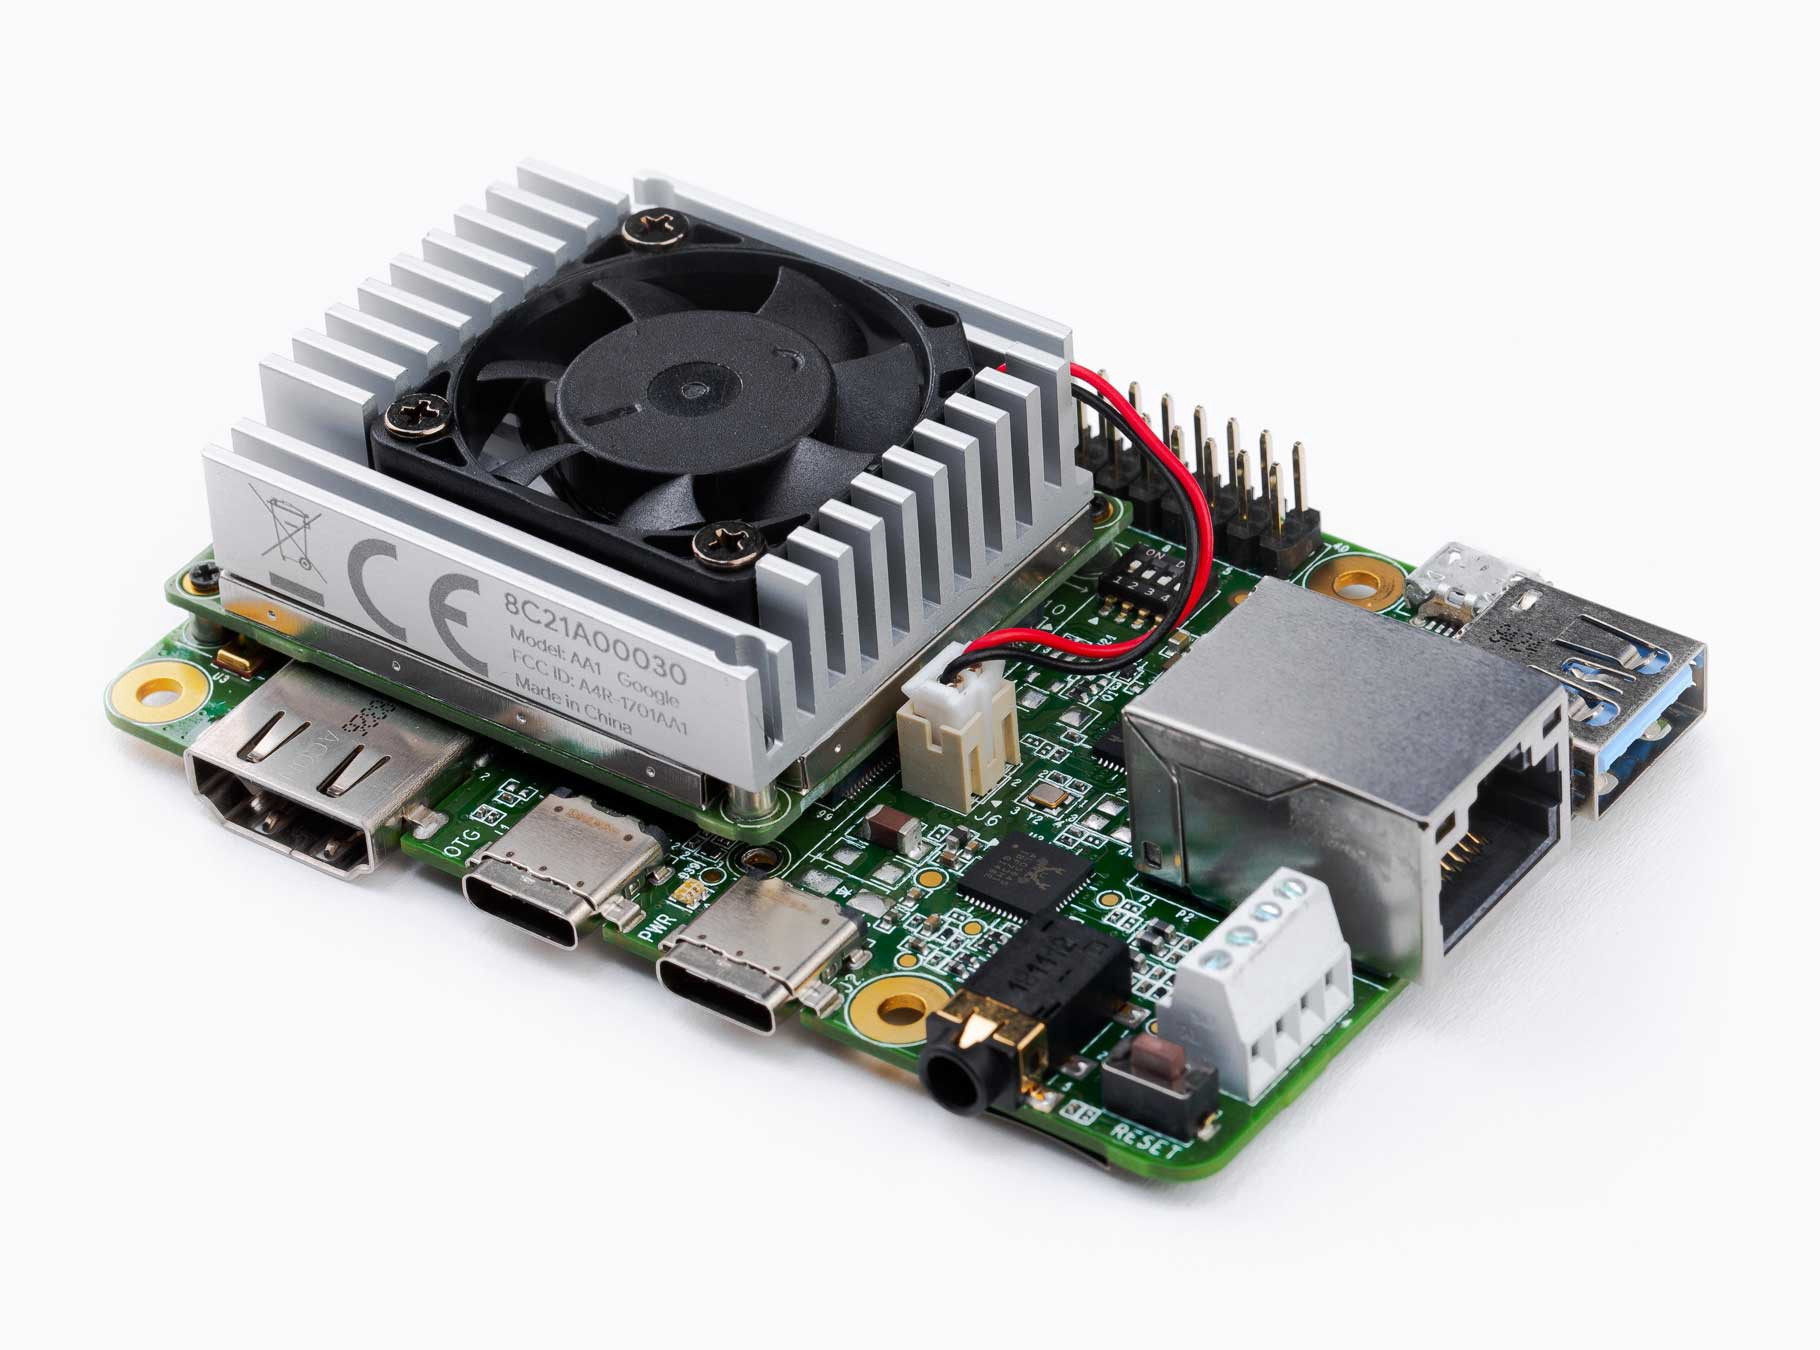
\includegraphics[width=50mm,scale=0.5]{tpu}
		\caption{Some images}\label{fig:foobar}
	\end{figure}
\end{frame}

\section{Hardware Comparison CPU vs GPU}
\begin{frame}
	\frametitle{Hardware Comparison CPU vs GPU}
	\subsection{Hardware Comparison CPU vs GPU}
	\begin{figure}
		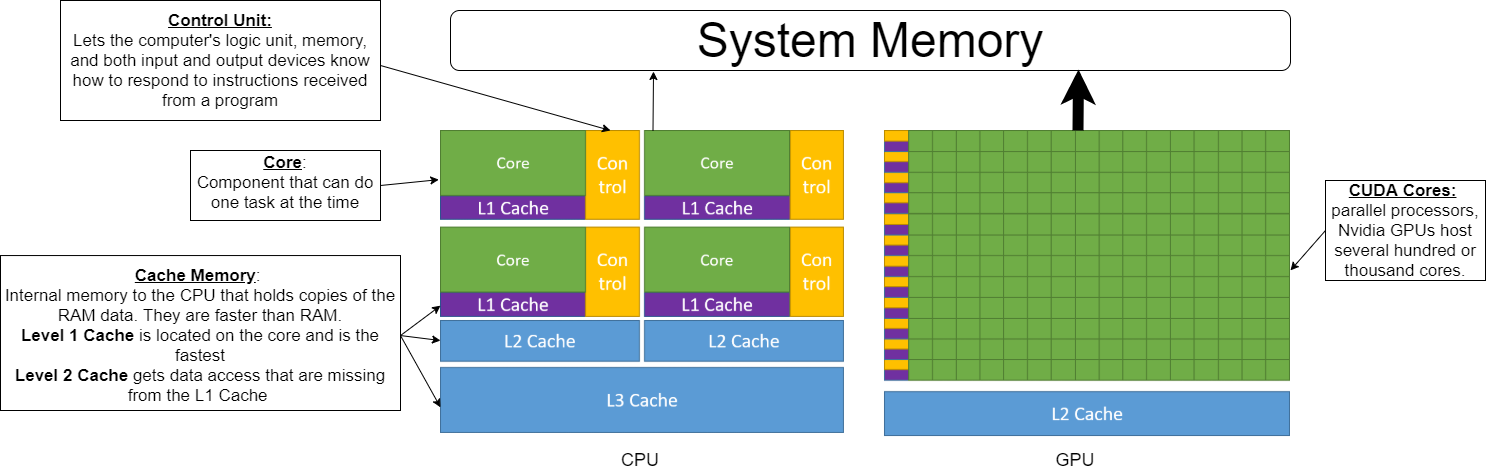
\includegraphics[width=\textwidth,height=\textheight,keepaspectratio]{cpu_vs_gpu}
	\end{figure}
\end{frame}

\begin{frame}
	\frametitle{Hardware Comparison CPU vs GPU}
	\begin{center}
		\begin{tabular}{| c | c | c |}
			\hline
			\textbf{Processor Type} & \textbf{CPU} & \textbf{GPU} \\ 
			\hline
			\textbf{Processor Model} & 	i9 7980XE & Tesla V100 \\  
			\textbf{Manufacturer} & Intel & Nvidia  \\
			\textbf{Processor Speed (Max)} &  \textbf{4.3 GHz}& 1.380 GHz  \\
			\textbf{Memory (up to)} & \textbf{128 GB (RAM)} & 32 GB (GRAM) \\
			\textbf{Number of Cores} & 18 & \textbf{5120 (CUDA cores)} \\
			\textbf{Single Precision  GFLOPS} & 13.1 & \textbf{148.992} \\
			\textbf{Memory Bandwidth} & 45.8 GB/s & \textbf{900 GB/s}\\
			\textbf{Price} & \textasciitilde \textbf{R 16 000} & \textasciitilde R 200 000\\
			\hline  
		\end{tabular}
	\end{center}
\end{frame}

\section{NVidia GPUs - CUDA APsI}
\begin{frame}
	\frametitle{NVidia GPUs - CUDA API}
	\begin{center}
\begin{itemize}
	\item CUDA is a parallel computing platform and programming model developed by NVIDIA for general computing on graphical processing units (GPUs). With CUDA, developers are able to dramatically speed up computing applications by harnessing the power of GPUs.
	\item CUDA is a programming language that uses the Graphical Processing Unit (GPU). 
	\item Its is an extension of C++, to provide basic instructions to GPU CUDA cores. The developer needs to be very much aware of C++ Memory Management for best performance.
\end{itemize}
	\end{center}
\end{frame}

\begin{frame}
	\frametitle{NVidia GPUs - CUDnn}
	Deep Learning specific CUDA GPU-accelerated library for  deep neural network routines likes:
	\begin{center}
		\begin{itemize}
			\item Back-and-forth Cross-correlation and/or convolution, neuron activations, pooling ,batch normalization
			\item Tensor transformations
			\item Equivalent: BLAS, cuBLAS, Eigen
		\end{itemize}
	\begin{figure}
	
\includegraphics[width=\textwidth,height=\textheight,keepaspectratio]{dl_logos_wide_002}
\end{figure}
	\end{center}
\end{frame}

\begin{frame}
	\frametitle{NVidia GPUs - CUDnn}
	\begin{center}
		\begin{figure}
			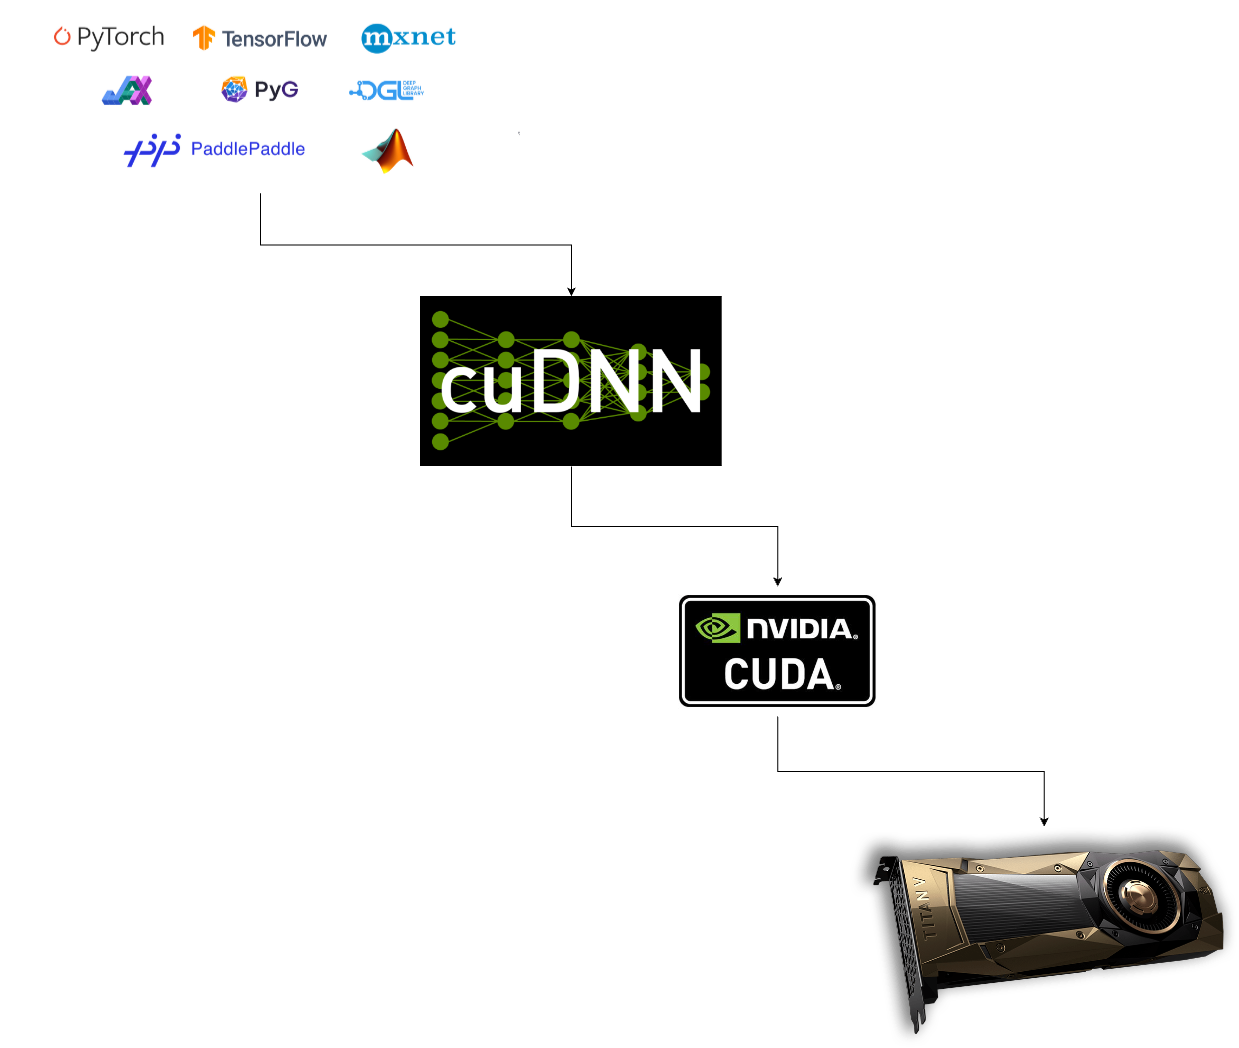
\includegraphics[width=\textwidth,height=\textheight,keepaspectratio]{DL_Stack_3}
		\end{figure}
	\end{center}
\end{frame}


\begin{frame}
	\frametitle{Tensors: Operations - Addition}
	%\subsection{Addition}
		 \begin{figure}
		\includegraphics[scale=0.17]{"1 - original_image"}
		\caption{Original Image}
	\end{figure}
\end{frame}

\begin{frame}
	\frametitle{Tensors: Operations - Addition}
	%\subsection{Addition}
	\begin{figure}
		\includegraphics[scale=0.17]{"2 - gauss_noise"}
		\caption{Noise}
	\end{figure}
\end{frame}

\begin{frame}
	\frametitle{Tensors: Operations - Addition}
	%\subsection{Addition}
	\begin{figure}
		\includegraphics[scale=0.17]{"3 - gn_img"}
		\caption{Image + Noise}
	\end{figure}
\end{frame}

\begin{frame}
	\frametitle{Tensors: Operations - Addition}
	%\subsection{Addition}
	\begin{figure}
		\includegraphics[scale=0.17]{"4 - gn_img_avg"}
		\caption{(Image + Noise) + Image}
	\end{figure}
\end{frame}

\begin{frame}
	\frametitle{Tensors: Operations - Matrix Multiplication}
	%\subsection{Matrix Multiplication}
\begin{itemize}
	\item The most used operation in Machine Learning/Deep Learning
	\item There are many types of Matrix Multiplication of \textit{\textbf{MatMul}}. There 3 are the most common matrix multiplication:
	\begin{itemize}
		\item Brute Force Multiplication
		\item Column-Wise Multiplication
		\item Block Multiplication		
	\end{itemize}
\end{itemize}
\end{frame}

\begin{frame}
	\frametitle{Tensors: Operations - Matrix Multiplication}
	%\subsection{Matrix Multiplication}
	\begin{figure}
		\includegraphics[scale=0.17]{"1 - original_image"}
		\caption{Image}
	\end{figure}
\end{frame}

\begin{frame}
	\frametitle{Tensors: Operations - Matrix Multiplication}
	%\subsection{Matrix Multiplication}
	\begin{figure}
		\includegraphics[scale=0.17]{"conv_1"}
		\caption{Convolution 1}
	\end{figure}
\end{frame}

\begin{frame}
	\frametitle{Tensors: Operations - Matrix Multiplication}
	%\subsection{Matrix Multiplication}
	\begin{figure}
		\includegraphics[scale=0.17]{"conv_2"}
		\caption{Convolution 2}
	\end{figure}
\end{frame}

\begin{frame}
	\frametitle{Tensors: Operations - Matrix Multiplication}
	
	\begin{figure}
		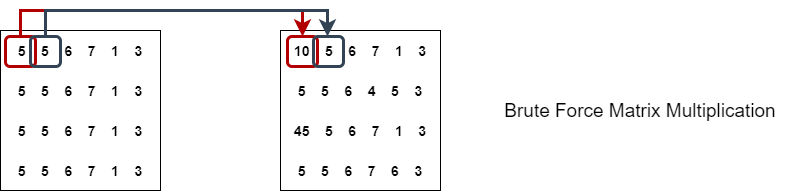
\includegraphics[width=100mm,scale=0.5]{brute_force_mat_mul}
		\\[\smallskipamount]
		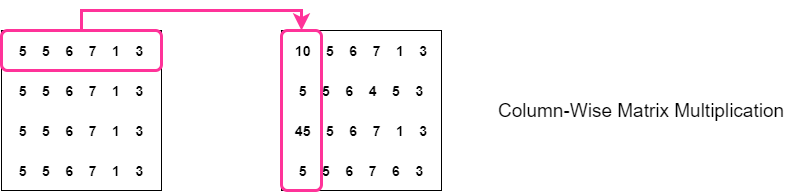
\includegraphics[width=100mm,scale=0.5]{column_wise_mat_mul}
		\\[\smallskipamount]
		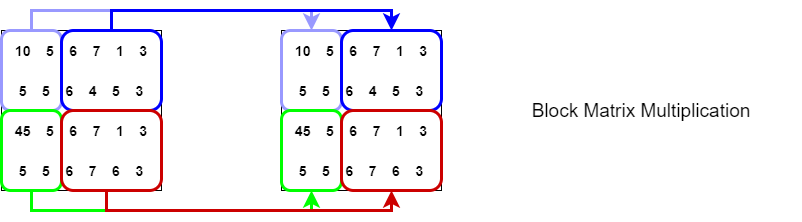
\includegraphics[width=100mm,scale=0.5]{block_multiplication}
	\end{figure}
	
%			\begin{figure}
%				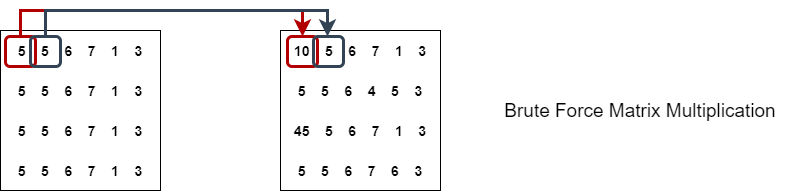
\includegraphics[width=50mm,scale=0.5]{brute_force_mat_mul}
%			\end{figure}
%
%			\begin{figure}
%				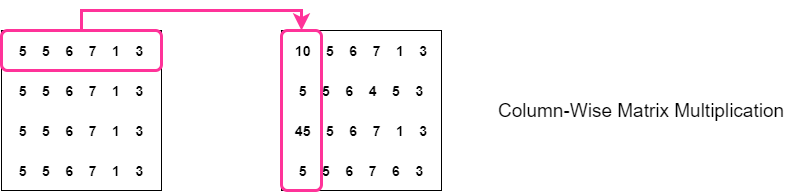
\includegraphics[width=50mm,scale=0.5]{column_wise_mat_mul}
%			\end{figure}
%
%			\begin{figure}
%				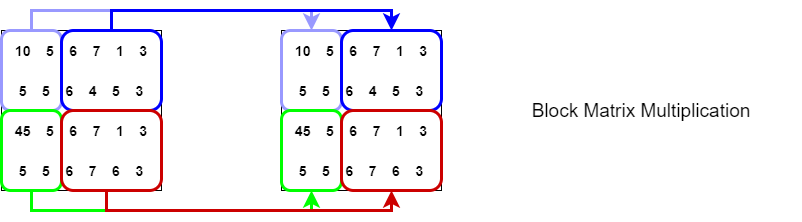
\includegraphics[width=40mm,scale=0.5]{block_multiplication}
%			\end{figure}
\end{frame}

\begin{frame}
	\frametitle{Tensors: Operations - Matrix Multiplication}
	\centering
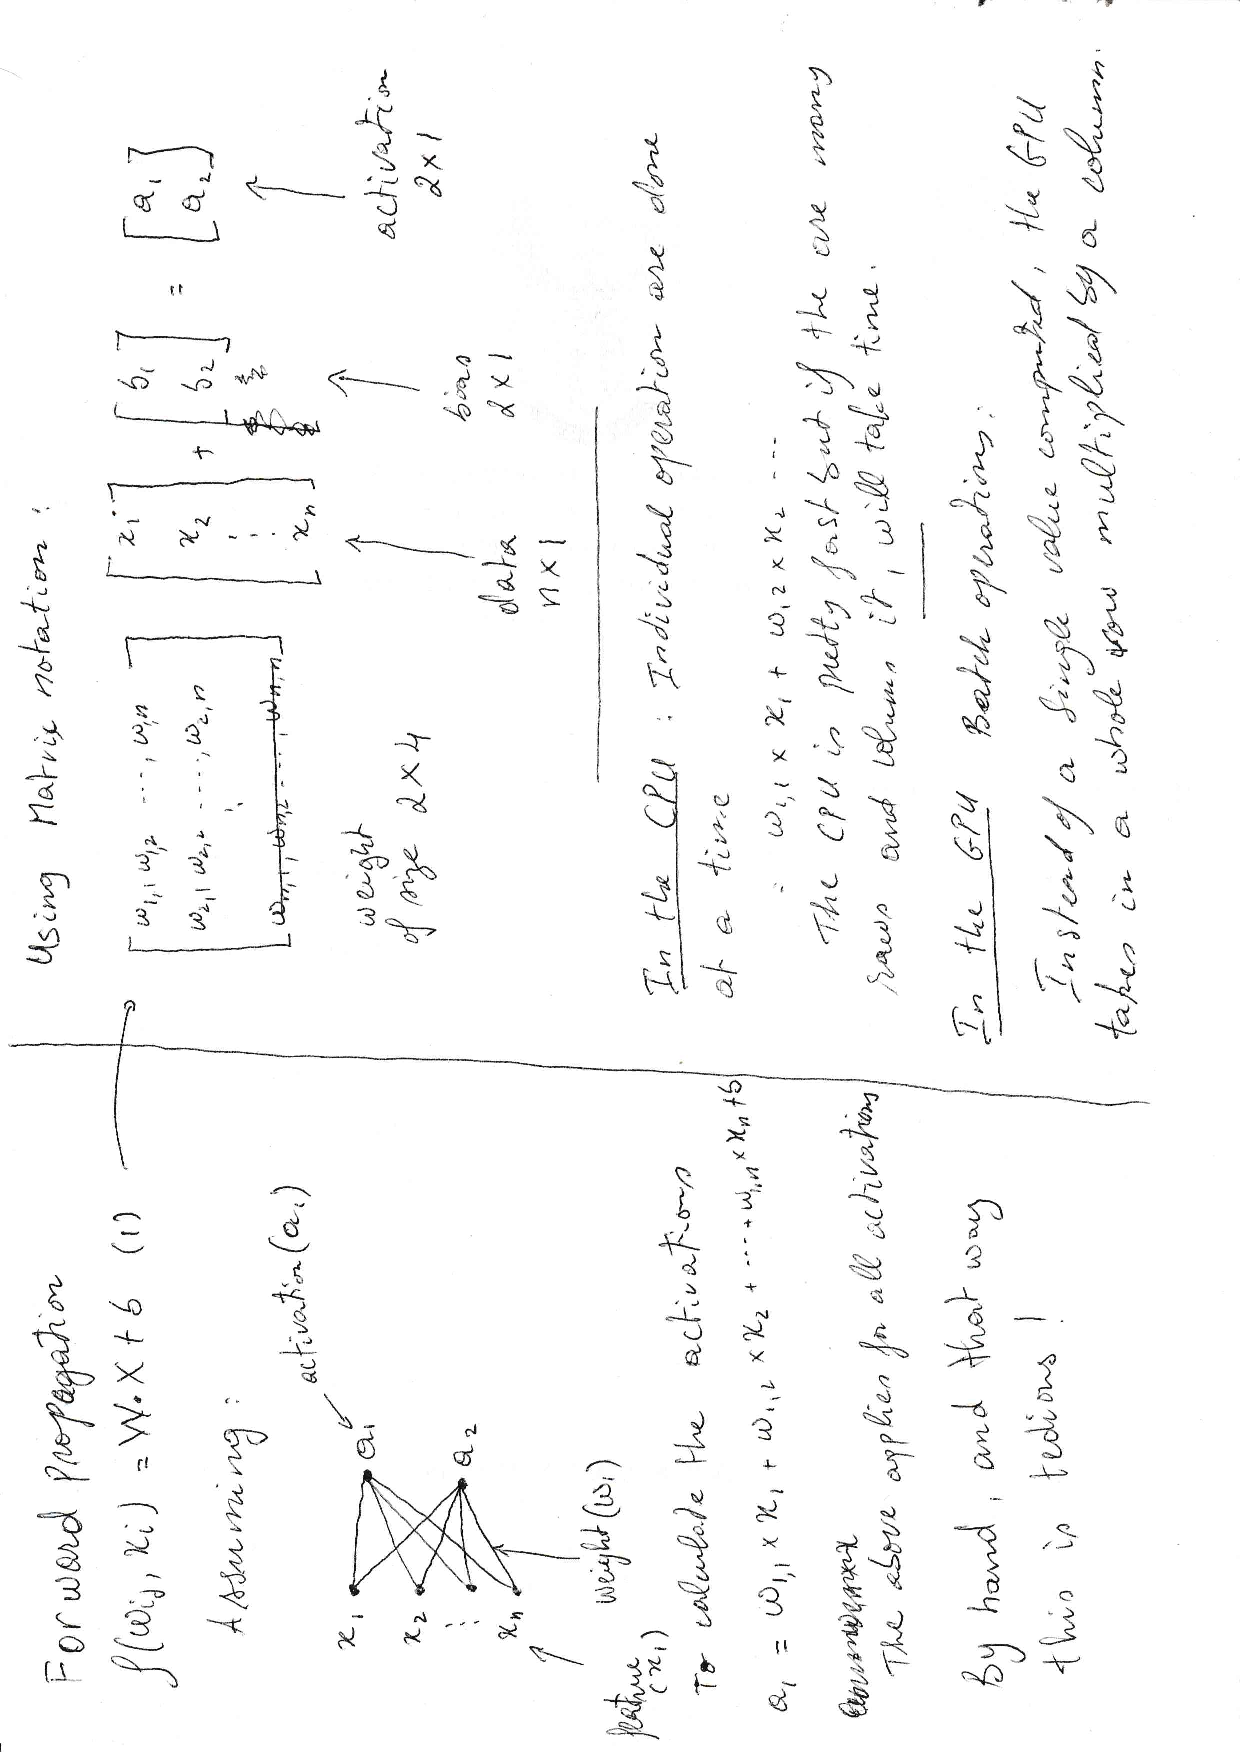
\includegraphics[width=\textwidth+2cm,height=\textheight+2cm,keepaspectratio, angle = -90 ]{demo.pdf}
\end{frame}

\section{Tensor Operations on Hardware}
\begin{frame}{movie}
	\frametitle{Matrix Computation on GPU vs CPU}
	\subsection{Matrix Computation on GPU vs CPU}
	\begin{figure}[h!]
	\centering
	{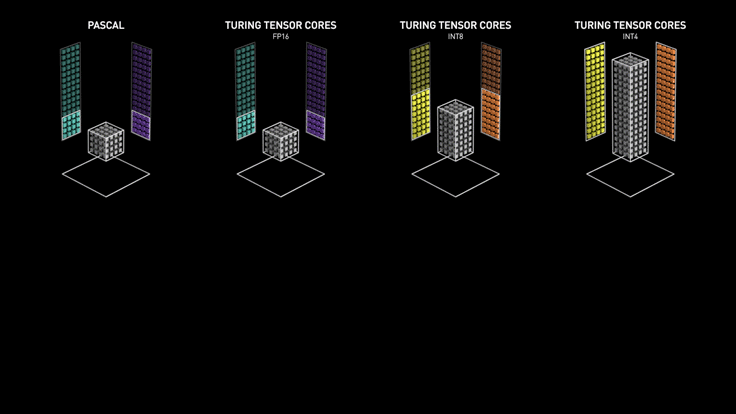
\includegraphics[width=1.0\textwidth]{gpugif.png}}
	\end{figure}
\end{frame}

\section{How does GPU works "faster" than the CPU?}
\begin{frame}
	\frametitle{How does GPU works "faster" than the CPU?}
	\begin{itemize}
		\item \textbf{Larger memory bandwidth}: More data can get in and out the component at a time,
		\item \textbf{Parallelization}: Those many CUDA cores work well in parallel for one given task
		\item \textbf{Fast Memory access}: Multiple L1 and L2 Cache memory,
		\item CUDA API allows you not to worry about memory allocation or deallocation, type of Matrix Multplication to use or how to orchestrate the parallelism of the cores. Some popular frameworks using CUDA:
	\end{itemize}
\end{frame}

\section{Very short demo}
\begin{frame}[fragile]
	\frametitle{Demo}
	
	We will run short 2 experiments on both the CPU and the GPU:
	\begin{itemize}
		\item Multiplication of 2 scalar: 8.8 x 8.9
		\item Multiplication of 2 relatively big matrices
	\end{itemize}
	
		\centering
	Demo Link: 
\href{https://colab.research.google.com/drive/1q32stN5vWQ3XApmu58BczJJy62wTI3Zf#scrollTo=UjuLyp2wMK7D}{Colab Experiment}.
\end{frame}

\section{References and Extended Reading}
\begin{frame}[fragile]
	\frametitle{References and Extended Reading (Links)}
	
	\begin{itemize}
\item \href{https://openmetal.io/docs/product-guides/private-cloud/gpu-parallel-computing/#GPU-Parallel-Computing}{GPU-Parallel-Computing}
\item \href{https://www.run.ai/guides/multi-gpu/cpu-vs-gpu#hpc}{CPU-vs-GPU 1}
\item \href{https://linuxhint.com/cpu-vs-gpu/#:~:text=While%20a%20CPU%20is%20the,ignited%20a%20worldwide%20AI%20boom.}{CPU-vs-GPU 2}
\item \href{https://cloud.google.com/tpu/docs/tpus}{TPU}
\item \href{https://codelabs.developers.google.com/codelabs/keras-flowers-data/#2}{Keras}
\item \href{https://cloud.google.com/blog/products/ai-machine-learning/an-in-depth-look-at-googles-first-tensor-processing-unit-tpu}{TPU}
\item \href{https://developer.nvidia.com/cuda-zone#:~:text=CUDA%C2%AE%20is%20a%20parallel,harnessing%20the%20power%20of%20GPUs.}{CUDA}
\item \href{https://developer.nvidia.com/blog/even-easier-introduction-cuda/}{Intro to CUDA}
\item \href{https://www.run.ai/guides/nvidia-cuda-basics-and-best-practices/nvidia-cudnn}{CUDnn}
\item \href{https://phucnsp.github.io/blog/self-taught/2020/03/22/self-taught-pytorch-part1-tensor.html}{Fundamental DL: Pytorch}
\item \href{https://www.gpuzoo.com/Compare/NVIDIA_Tesla_V100_SMX2__vs__NVIDIA_Titan_V/}{NVidia Titan V}
\item \href{https://www.intel.com/content/www/us/en/developer/articles/news/raw-compute-power-of-new-intel-core-i9-processor-based-systems-enables-extreme-megatasking.html#:~:text=The%20new%20Intel%C2%AE%20Core,should%20calculate%20to%201.3%20teraflops.}{i9}
	\end{itemize}
	
\end{frame}

\end{document}